\subsection{R-2R-Netzwerk} % (fold)
\label{sub:R-2R-Netzwerk}
\begin{frame}
    \frametitle{R-2R-Netzwerk}
    \framesubtitle{}
    \begin{figure}[H]
        \begin{center}
                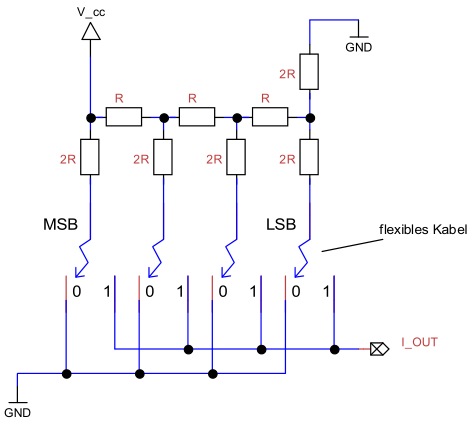
\includegraphics[scale=0.5]{./img/schaltung/r2r_0.png}
        \end{center}
    \end{figure}
\end{frame}

\begin{frame}
    \frametitle{Funktionsweise}
    \framesubtitle{}
    \begin{columns}[c]
        \column{0.7\textwidth}
            \begin{block}{}
                \begin{gather*}
                    I_{out} = \frac{U_{in}}{2R}\left( \frac{x_0}{8} +
                    \frac{x_1}{4} + \frac{x_2}{2} + \frac{x_3}{1} \right) \\
                    U_{out} = - U_{in} \frac{x}{x_{max} +1}
                \end{gather*}
                \begin{itemize}
                    \item lineare Schaltung 
                    \item 4-bit Zahl bestimmt Ausgangsstrom und Spannung
                \end{itemize}
            \end{block}
        \column{0.3\textwidth}
            \begin{figure}[H]
                 \begin{center}
                         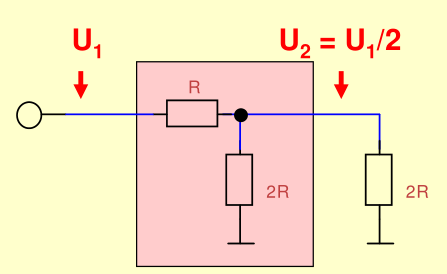
\includegraphics[scale=0.2]{./img/schaltung/r2r_1.png}
                 \end{center}
            \end{figure}
            \begin{figure}[H]
                 \begin{center}
                         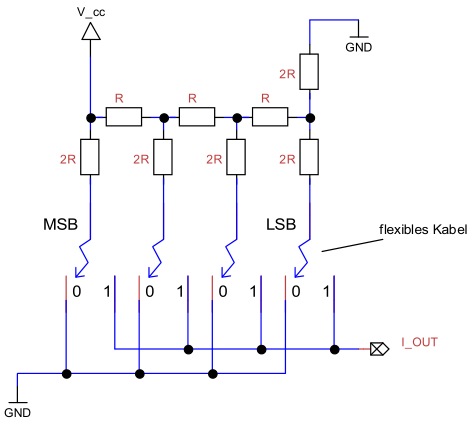
\includegraphics[scale=0.2]{./img/schaltung/r2r_0.png}
                 \end{center}
            \end{figure}
    \end{columns}
\end{frame}

\begin{frame}
    \frametitle{Messwerte}
    \framesubtitle{}
    \begin{figure}[H]
    \begin{center}
            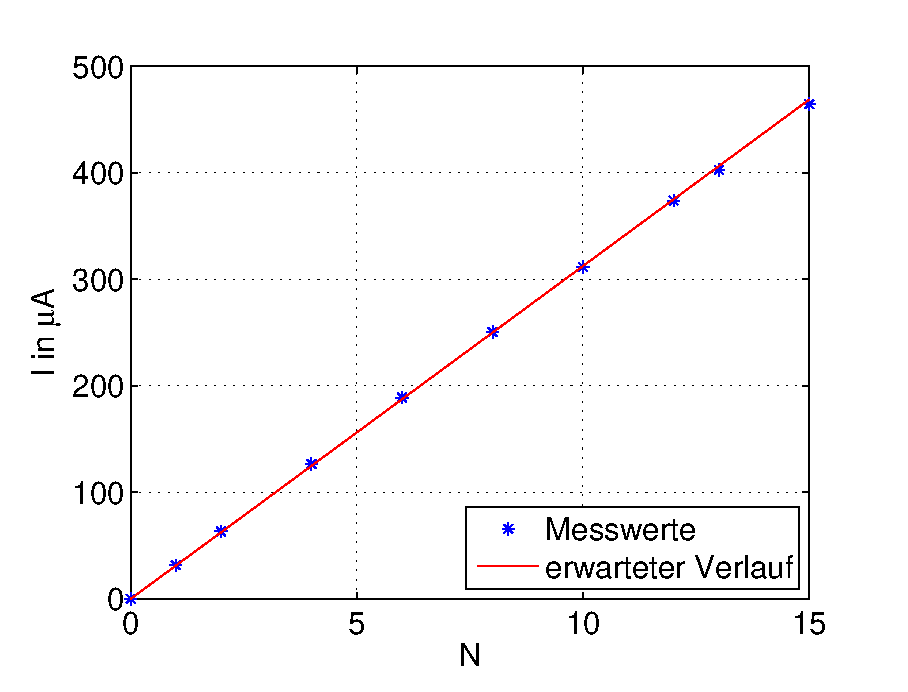
\includegraphics[scale=0.37]{./img/graph/Aufgabe1a.eps}
    \end{center}
    \end{figure}
    \begin{block}{Theorie}
         \begin{itemize}
            \item linearer Verlauf $\rightarrow$ für Theoriekurve ist
            nur $I_{max}$ nötig
            \begin{equation*}
                I_{max} = \frac{U_{in}}{2R}\left( \frac{1}{8} +
                \frac{1}{4} + \frac{1}{2} + \frac{1}{1} \right) 
                = \frac{15U_{in}}{16R}
                = 458.75 \mu A
            \end{equation*}
            \begin{equation*}
                I_{Theorie} = 458.75 \mu A \cdot x
            \end{equation*}
         \end{itemize}
    \end{block}
\end{frame}

\begin{frame}
    \frametitle{Messwerte}
    \framesubtitle{}
    \begin{figure}[H]
    \begin{center}
            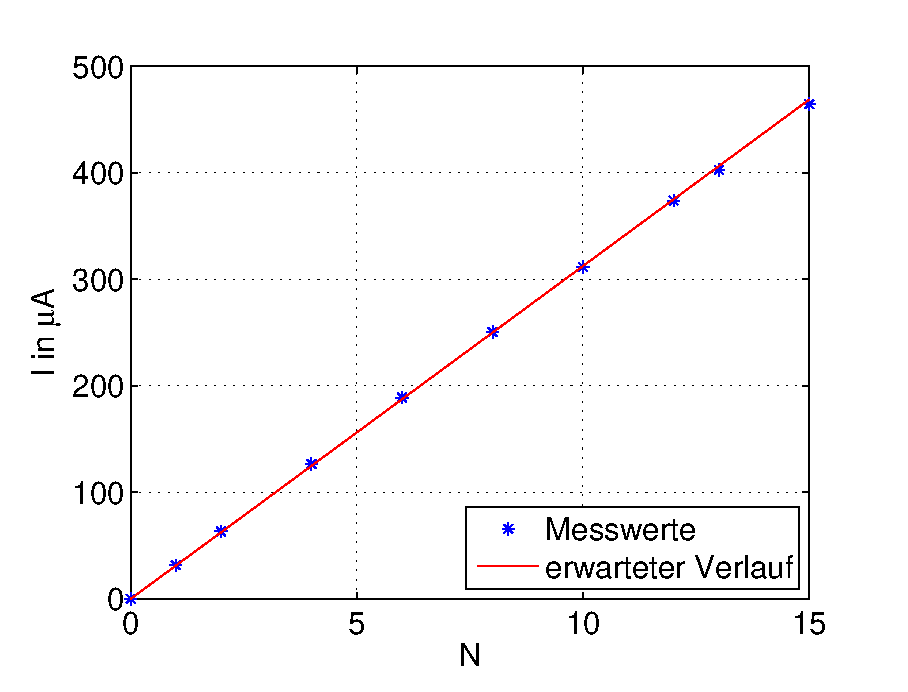
\includegraphics[scale=0.37]{./img/graph/Aufgabe1a.eps}
    \end{center}
    \end{figure}
    \begin{alertblock}{}
        \begin{center}
            Eigentlich ist die Theoriekurve stufenförmig!
        \end{center}
    \end{alertblock}
\end{frame}

\begin{frame}
    \frametitle{Messwerte}
    \framesubtitle{}
    \begin{figure}[H]
        \begin{center}
                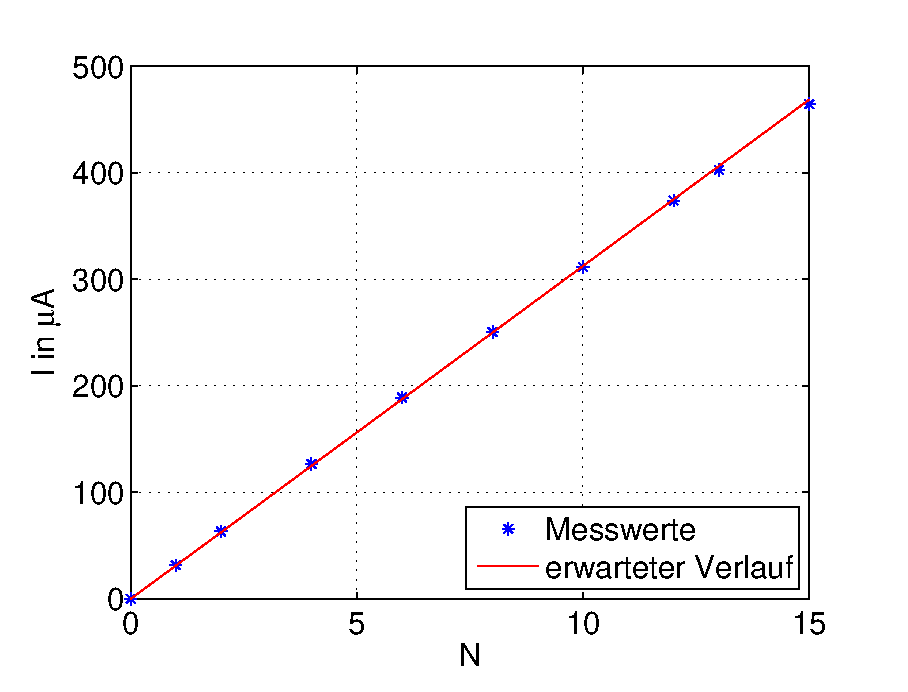
\includegraphics[scale=0.5]{./img/graph/Aufgabe1a.eps}
        \end{center}
    \end{figure}
    \begin{block}{Messung}
        \begin{itemize}
            \item Nullpunktsfehler: $0.003 \mu A$
            \item Sehr guter linearer Verlauf
        \end{itemize}
    \end{block}
\end{frame}

% subsection R-2R-Netzwerk (end)
